\documentclass[10pt]{article}
\usepackage{hyperref}
\usepackage{amsmath}
\usepackage{tikz}
\usepackage{qtree}
\usepackage{tikz-qtree}
\usepackage{pgfplots}
\usepackage{listings}
\usepackage{amsmath}
\usepackage{amsfonts}
\usepackage{amssymb}
\definecolor{light-gray}{gray}{0.95}
\usepackage{listings}
\lstset{
    numbers=left,
    breaklines=true,
    backgroundcolor=\color{light-gray},
    tabsize=2,
    basicstyle=\ttfamily,
}
\usepackage{setspace}
\renewcommand{\baselinestretch}{1.3} 
\usepackage{graphicx}
\usepackage[export]{adjustbox}
\usepackage{amsmath,amssymb,amsthm}
\usepackage{fancyhdr}
\renewcommand{\baselinestretch}{1.34} 
\usepackage{geometry}
\usepackage{enumitem}
\usepackage{algorithm}
\usepackage{algpseudocode}
\usepackage{multicol}


\setlength{\parindent}{0pt}
\setlength{\parskip}{5pt plus 1pt}
\setlength{\headheight}{13.6pt}
\newcommand\question[1]{\vspace{1.2em}\hrule\textbf{ #1}\vspace{.5em}\hrule}
\renewcommand\part[1]{\vspace{.10in}\textbf{#1)} \enspace}
\pagestyle{fancyplain}
\fancyhf{}
\renewcommand{\headrulewidth}{1.4pt}
\lhead{\textbf{\ANDREWID }}
\cfoot{\textbf{First Draft } - \thepage   }
\rhead{\rule[-1ex]{0pt}{3.5ex} Hossein Naderi }
\newcommand\ANDREWID{Distributed Queue using $\Omega(\log n)$ Shared Memory Accesses} 
\newcommand\HWNUM{1}
\newtheorem{theorem}{Theorem}
\newtheorem{lemma}[theorem]{Lemma}
\theoremstyle{definition}
\newtheorem{definition}{Definition}

\begin{document}

\question{Introduction}

Queue (Q): We are going to implement a MEMD Queue using T.

CAT Tree (CAT): A tree for storing some operation on Q by order. Every leaf  In each node there is a tuple stores (\#enqueues, \#dequeues, \#null response dequeues) of the node's subtree.

\begin{center}
\Tree [.$op_1,op_2,op_3,op_4,op_5$ [.$op_1,op_2$ $op_1$ $op_2$ ]
          [.$op_3,op_4,op_5$ $op_3$
               [.$op_4,op_5$ $op_4$ $op_5$ ] ] ]
\end{center}

In order to compute $deq_i$ faster we augment the tree with these parameters. At each node we store

Tournament Tree (T): Each process is assigned to one of the Tournament Tree leaves. Every node contains a pointer to a node of the CAT Tree.
\begin{center}
\Tree [.$root$ [.$n$ [.$n$ $p_1$ $p_2$ ] [.$n$ $p_3$ $p_4$ ] ]
          [.$n$ [.$n$ $p_5$ $p_6$ ] [.$n$ $p_7$ $p_8$ ] ] ]
\end{center}

Each node in the Tournament Tree points to a node in the CAT tree.

\begin{center}
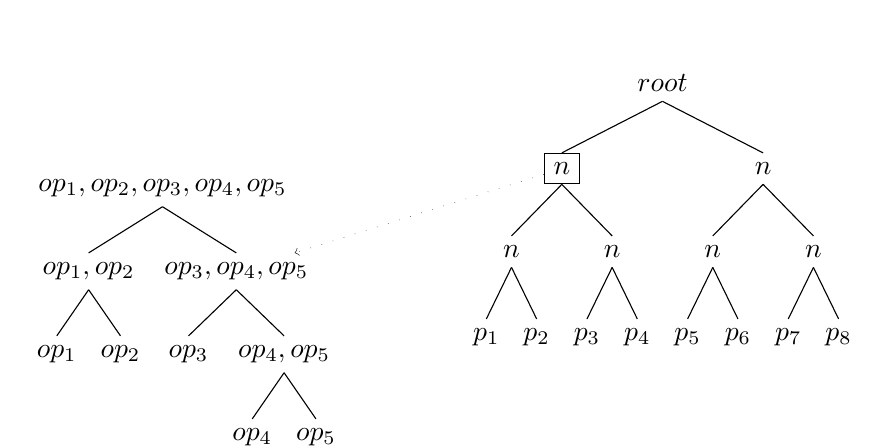
\begin{tikzpicture}
\Tree [.$op_1,op_2,op_3,op_4,op_5$ [.$op_1,op_2$ $op_1$ $op_2$ ]
          [.\node(site){$op_3,op_4,op_5$}; $op_3$
               [.$op_4,op_5$ $op_4$ $op_5$ ] ] ]
\begin{scope}[shift={(2.5in,0.5in)}]
\Tree [.$root$ [.\node[draw](root){$n$}; [.$n$ $p_1$ $p_2$ ] [.$n$ $p_3$ $p_4$ ] ]
          [.$n$ [.$n$ $p_5$ $p_6$ ] [.$n$ $p_7$ $p_8$ ] ] ]
\end{scope}
\draw[very thin, loosely dotted, ->](root)--(site);
\end{tikzpicture}
\end{center}

\pagebreak

\question{Algorithm}

Our idea is to replace the strings in our universal construction with trees in order to make \textsc{DO()} operations faster. Since for $dequeue$ queries you only have to know that earliest element added (if it exists). We told earlier the ordering of operations in the CAT tree before.

\question{Merging children of node $n$}											



In each node of CAT tree all the propagated operations are descendants of its left child and all not propagated operations are descendants of the right child.

\begin{center}
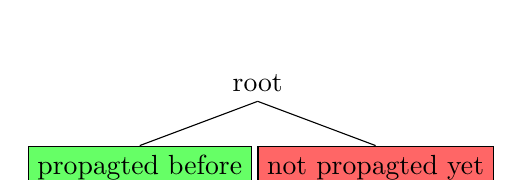
\begin{tikzpicture}
        \Tree [ .root \node[draw,fill=white!40!green]{propagted before}; \node[draw,fill=white!40!red]{not propagted yet}; ]
\end{tikzpicture}
\end{center}



Initial Configuration:

\begin{center}
\begin{tikzpicture}[sibling distance=30pt]

\Tree [ .\node(nnode){$n$}; [.\node(lnode){$l$}; ... ] [ .\node(rnode){$r$}; ... ] ]

\begin{scope}[shift={(-1in,-0.7in)}]
\Tree [.\node(lst){$*l$}; \node[draw]{$P_l$}; \node[draw]{$N_l$}; ]
\end{scope}

\begin{scope}[shift={(1in,-0.7in)}]
\Tree [.\node(rst){$*r$}; \node[draw]{$P_r$}; \node[draw]{$N_r$}; ]
\end{scope}

\begin{scope}[shift={(0in,-1.3in)}]
\Tree [.\node(nst){$*r$}; \node[draw]{$P_r \cup P_l$}; \node[draw]{$N_n$}; ]
\end{scope}

\draw[thin, loosely dotted, ->](nnode)--(nst);
\draw[thin, loosely dotted, ->](lnode)--(lst);
\draw[thin, loosely dotted, ->](rnode)--(rst);

\end{tikzpicture}
\end{center}

After Merging:

\begin{center}
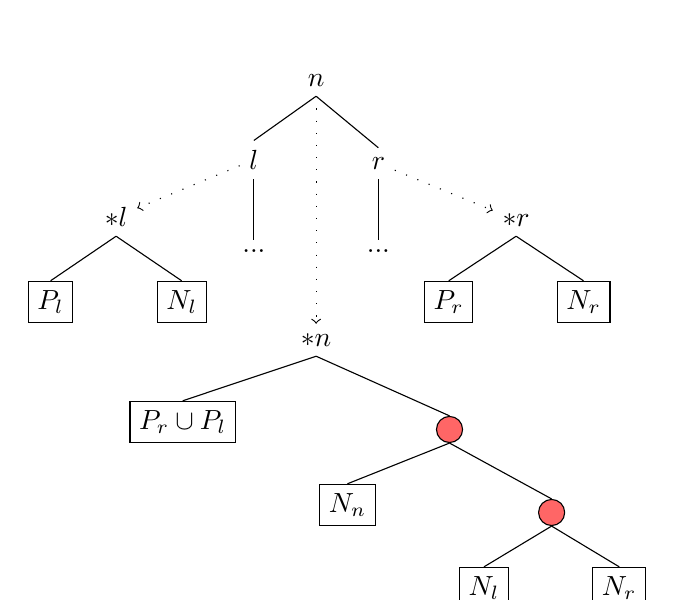
\begin{tikzpicture}[sibling distance=30pt]

\Tree [ .\node(nnode){$n$}; [.\node(lnode){$l$}; ... ] [ .\node(rnode){$r$}; ... ] ]

\begin{scope}[shift={(-1in,-0.7in)}]
\Tree [.\node(lst){$*l$}; \node[draw]{$P_l$}; \node[draw]{$N_l$}; ]
\end{scope}

\begin{scope}[shift={(1in,-0.7in)}]
\Tree [.\node(rst){$*r$}; \node[draw]{$P_r$}; \node[draw]{$N_r$}; ]
\end{scope}

\begin{scope}[shift={(0in,-1.3in)}]
\Tree [.\node(nst){$*n$}; \node[draw]{$P_r \cup P_l$};
      [ .\node[circle, draw, fill=white!40!red]{}; \node[draw]{$N_n$};
      [ .\node[circle, draw, fill=white!40!red]{}; \node[draw]{$N_l$}; \node[draw]{$N_r$}; ] ] ]
\end{scope}

\draw[thin, loosely dotted, ->](nnode)--(nst);
\draw[thin, loosely dotted, ->](lnode)--(lst);
\draw[thin, loosely dotted, ->](rnode)--(rst);

\end{tikzpicture}
\end{center}




\begin{algorithm}
\caption{Main Algorithm}\label{alg}
\begin{algorithmic}[1]
\begin{multicols}{2}


\Statex Shared Objects
\Statex \hspace{\algorithmicindent}Tournament Tree
\Statex \hspace{\algorithmicindent}CAT Tree
\Statex Local Objects
\Statex

\Function{Do}{operation op} 
\State l= p's assigned leaf in tree
\State \Call{Add$_l$}{op}
\State \Call{Propagate}{l.parent}
\State \Return \Call{Compute}{op}
\EndFunction

\Statex

\Function{Propagate}{node n}
\Statex\Comment{Propagates $n$ operations    \,\,\,\,\,\,\,}
\If{n==root} \Return
\Else \State d=\Call{Merge}{n}
%\If{!\Call{Refresh}{n}}
%\State \Call{Refresh}{n} \EndIf
\EndIf
\State \Call{Propagate}{n.parent}
\EndFunction

\Statex

\Function{Merge}{node n}
\Statex\Comment{Merges two children of $n$ \& updates n*, augmented values}
\EndFunction

\Statex
\Function{Compute}{op}
\If{op.type=enq}\State\Return{}
\Else \Return{$enq_{\#enqs(op.l)-\#effective-deqs(op.l)}$}\EndIf
\EndFunction

\Statex
\Function{enqs}{l}
\Statex\Comment{Returns \#enqs before l}
\EndFunction

\Statex
\Function{enq}{i}
\Statex\Comment{Returns $enq_i$}
\EndFunction


\end{multicols}
\end{algorithmic}
\end{algorithm}

\question{Correctness}
TODO

\end{document}
